  \section{Introduction}
  This paper will explore serverless architecture by creating a static website and using a serverless compute service to provide a backend functionality. The practical element of this paper will deploy a sample web app, known as \textit{Wild Rydes}, provided by AWS. This site allows users to register, verify their email address and sign in after verification. Once authenticated the user can request a ride on a Unicorn by entering their location.
  
  The system will be implemented using a number of different AWS services:
  \begin{itemize}
    \item Static web content will be hosted on \textbf{S3};
    \item The backend functionality will be implemented using \textbf{Lambda};
    \item Authentication will be provided using \textbf{Amazon Cognito}, either through a self hosted \textbf{User Pool} of registered users, or sign in using a Google Identity;
    \item API endpionts will be created for the static website to trigger the backend serverless functions using \textbf{Amazon API Gateway};
    \item The data base for the system will be implemented using \textbf{DynamoDB}.
  \end{itemize}
  
  The use of these together in to architecture shown in \autoref{fig:architecture} allows the serverless implementation of \textit{MEAN stack-like} web app. Services and terms highlight above will be explored in the practical element.
  
    
  \begin{figure}[H]
    \caption{System Architecture}
    \centering
    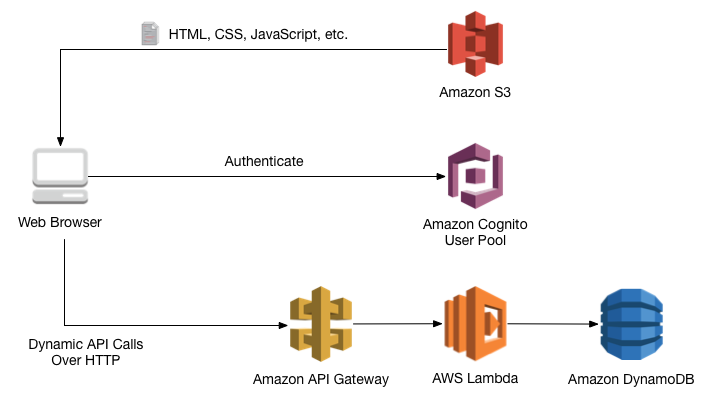
\includegraphics[width=0.8\textwidth,keepaspectratio]{system-architecture}
    \label{fig:architecture}
  \end{figure}
  
   
  \subsection{Objectives}
  Based on the above work to be completed the following objective have been outlined:
  
  \begin{itemize}
    \item Learn about serverless architecture;
    \item Implemented a serverless system using AWS Lambda;
    \item Explore possibility of creating a website backend using Amazon API gateway with Lambda;
    \item Examine the use of AWS Cognito for implementing user authentication using a hosted database of registered users and to examine signing in through social identity providers.
  \end{itemize} 
  
    \subsection{Background} 
    Prior to the introduction of serverless architectures, hosting web apps consisted of deploying the app to a server, either on premise or provided by a cloud service. For example, hosting a MEAN stack application on an AWS EC2 instance. This has the drawback of the financial cost of maintaining the server. Web apps may experience periods of inactivity. However, during these times the servers are still running and therefore continue to incur cost. There is also overhead involved with the provisioning and maintenance of the such servers and auto-scaling of the server. Serverless architectures aim to reduce the impact of these issues.
    
    The above example describes the a web app hosted on a server as this is the service which will be implemented as for the practical element of this paper. However, the same concepts, and alternative described below, apply to any code which a client may wish to run in the in the cloud via a provider.
    
      \subsubsection{Serverless Architecture}
      In a serverless model, a client does not need a server, either locally clouid provided to run  their code. Rather, the client provides only their code to a cloud provider which runs the code for them. The provider manages the execution of this code. Thus, it is often described as Function-as-a-Service (FaaS) as the cloud provider completely abstracts the servers away from the clients. Therefore the client does not have to provision or maintain any servers \citep{stackify}.
      
      It is important to note that serverless computing is not a client uploading some code, running and reading a response or results. The client provides the code and it is run whenever necessary. Hence, serverless computing is described as being an event driven execution model. The code is provided by the client and the execution and life-cycle management of a function is maintained by the provider after being triggered by some event. \citep{kanso}. This will be demonstrated in this paper through the use of Amazon API gateway. The API endpoints will act as  triggers for the functions saved in the serverless architecture.
      
      These features of serverless computing provide a number of benefits over traditional server base computing.
      \begin{itemize}
        \item \textbf{No server administration:} Clients do not need to provision or maintain servers as the servers are abstracted away from them.
        \item \textbf{No autoscaling: } Clients do not need to configure autoscaling of their servers to adjust to  traffic bursts as the provider completely manages the backend servers.
        \item \textbf{Reduced costs:} Clients pay only for execution time instead of paying to run servers constantly, even when not in use.
      \end{itemize}